% =============================================================
% AXIOM: A Binary Substring Graph for Zero-Error Retrieval
% IEEE conference format, two-column, 10pt
% Author: Yashas K
% Date: October 2026
% Target venue: IEEE Big Data 2027 or ACM CIKM 2027
%
% Compile: tectonic main.tex
% =============================================================

\documentclass[conference]{IEEEtran}

\usepackage{cite}
\usepackage{amsmath,amssymb,amsfonts}
\usepackage{algorithmic}
\usepackage{graphicx}
\usepackage{textcomp}
\usepackage{xcolor}
\usepackage{listings}
\usepackage{booktabs}
\usepackage{tabularx}
\usepackage{array}
\usepackage{url}
\usepackage{hyperref}

\hypersetup{
    colorlinks=true,
    linkcolor=blue!60!black,
    citecolor=blue!60!black,
    urlcolor=blue!60!black,
    pdftitle={AXIOM: A Binary Substring Graph for Zero-Error Retrieval},
    pdfauthor={Yashas K},
    pdfsubject={Exact substring retrieval, LZ77, hallucination prevention},
    pdfkeywords={exact retrieval, LZ77, RAG, hallucination, suffix tree}
}

\lstdefinelanguage{Rust}{
  keywords={fn, let, mut, struct, impl, for, in, while, if, else, return, match, Some, None, true, false, as, use, self, where, break, continue, const, enum, pub, ref, move},
  keywordstyle=\color{blue!70!black}\bfseries,
  ndkeywords={u8, u16, u32, u64, usize, i32, i64, f64, bool, Vec, HashMap, Option, String, str, Self},
  ndkeywordstyle=\color{teal!60!black}\bfseries,
  sensitive=true,
  comment=[l]{//},
  commentstyle=\color{gray!80!black}\itshape,
  stringstyle=\color{red!60!black},
  morestring=[b]",
}

\lstset{
  language=Rust,
  basicstyle=\ttfamily\footnotesize,
  showstringspaces=false,
  breaklines=true,
  frame=single,
  framesep=3pt,
  rulecolor=\color{gray!50},
  backgroundcolor=\color{gray!5},
  xleftmargin=4pt,
  xrightmargin=2pt,
  aboveskip=4pt,
  belowskip=4pt,
}

\begin{document}

\title{AXIOM: A Binary Substring Graph for Zero-Error Retrieval\\
\large An Honest Engineering Study on Real Gutenberg Text at 1, 10, and 100\,MB}

\author{
\IEEEauthorblockN{Yashas K}
\IEEEauthorblockA{Independent Researcher\\
Bangalore, India\\
ORCID: 0009-0005-8928-5341\\
Code: \url{https://github.com/Yashas-K-Gangatkar/axiom}}
}

\maketitle

\begin{abstract}
This paper presents \textbf{AXIOM}, a multi-layer binary substring graph for exact-match retrieval, and evaluates it honestly against standard compressors and classical data structures. AXIOM has three layers: V1, a prefix-sharing binary trie; V2, a Lempel-Ziv-77 (LZ77) macro graph that also shares middle substrings; and V3.1, a LOUDS succinct trie that reduces V1's storage by 94\%. We stress-test all three on real Project Gutenberg text at 1, 10, and 100\,MB and report every measurement directly. The headline result is a 0\% hallucination rate across all corpus sizes, verified against five adversarial fake queries per size. We also report, without omission, that AXIOM V2 is 38$\times$ worse than \texttt{xz -9} on compression ratio, that V1 bloats 212$\times$ on disk (solved by V3.1 LOUDS), and that substring search is $O(N{\cdot}L)$ rather than $O(L)$ because AXIOM does not yet implement a generalized suffix tree. The contribution is therefore not a better compressor or a faster search engine, but a different infrastructure layer that provides a property none of these systems have: \emph{exact} substring retrieval on binary data with shared-substring dedup across documents, applicable as a verification gate behind approximate nearest-neighbor (ANN) retrieval in retrieval-augmented generation (RAG) pipelines.
\end{abstract}

\begin{IEEEkeywords}
exact substring retrieval, LZ77, hallucination prevention, RAG, suffix tree, binary trie
\end{IEEEkeywords}

% =============================================================
\section{Introduction}
% =============================================================

Large language model (LLM) hallucination is often attributed to the model itself, but a substantial fraction of hallucinated retrievals originate one layer below, in the approximate nearest-neighbor (ANN) index that backs retrieval-augmented generation (RAG). ANN methods such as FAISS~\cite{johnson2019faiss}, ScaNN~\cite{guo2020scann}, and HNSW~\cite{malkov2018hnsw} trade recall for speed: a recall@10 of 0.95 is considered excellent, meaning 5\% of true top-10 results are missing on average. The missing neighbors are replaced by semantically close but textually different vectors, and the downstream LLM commits to the wrong passage. The model is blamed; the index that caused the error is not.

This paper investigates an alternative substrate: a retrieval graph that, by construction, cannot return a passage that is not present. We call it AXIOM. The name reflects the goal of \emph{axiomatic exactness}---no probability anywhere in the retrieval path. AXIOM has two layers. V1 is a binary trie of all chunks of a corpus with one node per bit. V2 is a Lempel-Ziv-77-style macro graph where repeated substrings of length $\geq 8$ bytes become shared macro chains, and each chunk is encoded as a sequence of literals and macro references. There is no hashing, no embedding, no probability. Retrieval is exact substring match. If a query has no exact match in the graph, the graph returns nothing.

We deliberately do not compare AXIOM to FAISS as a competitor. AXIOM answers a different question: ``does this exact substring appear in the corpus?'' FAISS answers ``which $k$ vectors are closest to this query vector?'' The two are complementary. A practical hybrid pipeline would use FAISS for candidate generation and AXIOM for verification, eliminating the hallucinated-retrieval failure mode without sacrificing FAISS's latency.

\subsection{Contributions}

\begin{enumerate}
\item \textbf{Two-layer architecture.} V1 is a prefix-sharing binary trie. V2 is a Lempel-Ziv-77-style graph with byte-level hash chains and 64-byte maximum match length. Both serialize to disk with explicit byte counts.
\item \textbf{Honest stress test on real text.} We evaluate on 1, 10, and 100\,MB corpora built from ten public-domain Project Gutenberg books. Every reported number---file size, node count, build time, search time, hallucination rate---is measured, not extrapolated.
\item \textbf{Real comparison to standard compressors.} We benchmark \texttt{gzip -9}, \texttt{xz -9}, and \texttt{bzip2 -9} on the same corpora and report the actual ratios. AXIOM V2 is 38$\times$ worse than \texttt{xz} on the 100\,MB corpus.
\item \textbf{Zero-error verification.} Five adversarial fake queries per corpus size are all rejected, giving a 0\% hallucination rate. This is the only strong claim.
\item \textbf{Honest limitations.} V1 bloats 212$\times$ on disk. Substring search is $O(N{\cdot}L)$, not $O(L)$. V2 only compresses when the corpus has repetition. We state these explicitly.
\end{enumerate}

\subsection{What AXIOM Is Not}

AXIOM is not a better compressor than \texttt{gzip} or \texttt{xz}---on unique text, V2 is 1.69$\times$ larger than raw. It is not a faster search engine than FAISS---FAISS returns in microseconds, AXIOM's deep-needle search takes milliseconds. It does not replace Transformer-based LLMs. The contribution is a complementary infrastructure layer with a property none of these systems have: exact substring retrieval on binary data.

% =============================================================
\section{Background and Related Work}
% =============================================================

\subsection{Approximate Nearest Neighbor Search}

FAISS~\cite{johnson2019faiss} introduced production-grade ANN over dense embeddings, with product quantization and inverted file indexing. ScaNN~\cite{guo2020scann} improved on FAISS with anisotropic vector quantization. HNSW~\cite{malkov2018hnsw} provides graph-based ANN with logarithmic query time on average. All three trade recall for speed: a recall@10 of 0.95 is excellent, meaning 5\% of true top-10 results are missing. In a RAG pipeline, this 5\% error rate is invisible to the user but directly produces hallucinated citations. ANN is the right tool when the goal is to find similar items fast; it is the wrong tool when the goal is to verify that an item exists.

\subsection{Suffix Trees and Suffix Arrays}

The suffix tree, introduced by Weiner~\cite{weiner1973} and made practical by Ukkonen's $O(n)$ online construction~\cite{ukkonen1995}, supports $O(L)$ substring search on a text of length $n$ for a pattern of length $L$. Suffix arrays~\cite{manber1993} reduce the memory footprint by a constant factor while preserving $O(L + \log n)$ search via binary search. These are the gold standard for exact substring retrieval. AXIOM's V1 is a degenerate suffix structure: a trie of all suffixes of all chunks, but without the suffix-link pointers that make suffix trees efficient. Adding suffix links is equivalent to upgrading V1 to a generalized suffix tree, which is the natural next step (Section~\ref{sec:future}).

\subsection{Lempel-Ziv Family}

LZ77~\cite{ziv1977lz77} introduced sliding-window substring matching: at each position, the encoder searches backwards for the longest match and emits a (offset, length) pair instead of a literal. LZSS~\cite{storer1982lzss} added a flag bit to distinguish literals from matches. LZMA (used by \texttt{xz}) adds range coding on top of LZ77. The V2 layer of AXIOM is, structurally, an LZ77 encoder with byte-level hash chains and a 64-byte maximum match length. There is no novelty in the compression algorithm itself; the contribution is in its application as a retrieval substrate where shared substrings are first-class nodes queryable by exact match.

\subsection{RAG Memory Layers}

LangChain, LlamaIndex, and Chroma each provide a memory layer that stores embedded chunks (typically 256--512 tokens each) in a vector database. Retrieval is ANN over these embeddings. The hallucination risk is well-documented~\cite{ji2023hallucination}: the model has no way to distinguish a correctly retrieved chunk from a near-miss. Some recent work adds verification~\cite{gao2023rag}, but this pushes verification back onto the model, which is itself the source of hallucination. AXIOM pushes verification down into the retrieval layer, where exactness is mathematically achievable.

% =============================================================
\section{AXIOM Architecture}
% =============================================================

\subsection{Design Principles}

AXIOM is built on three principles. First, \textbf{storage is binary}: the corpus is reduced to a stream of bits (8 bits per byte, MSB first), and the graph operates on bits. Second, \textbf{substrings are shared across documents}: when two chunks contain the same byte sequence, that sequence is stored once and referenced by both. Third, \textbf{retrieval is exact by construction}: every node pointer in the graph is a real address, never a hash bucket or an approximate match. There is no probability of returning a wrong answer because there is no probability anywhere in the system.

\subsection{V1: Prefix-Sharing Binary Trie}

V1 is a binary trie with one node per bit. Each node stores its bit value (0 or 1), two child pointers, and an end-of-string flag. Listing~\ref{lst:v1} shows the insertion algorithm.

\begin{lstlisting}[caption={V1 prefix-trie insertion.},label={lst:v1}]
fn insert_bits(&mut self, bits: &[u8]) -> u64 {
    let mut new_nodes: u64 = 0;
    let mut cur = self.root;
    for &b in bits {
        let child = if b == 0 { self.nodes[cur].child0 }
                    else { self.nodes[cur].child1 };
        cur = match child {
            c if c != u64::MAX => c,
            _ => {
                let n = self.new_node(b);
                new_nodes += 1;
                if b == 0 { self.nodes[cur].child0 = n; }
                else { self.nodes[cur].child1 = n; }
                n
            }
        };
    }
    self.nodes[cur].is_end = true;
    new_nodes
}
\end{lstlisting}

V1's trie structure means two chunks share nodes if and only if they share a prefix in their bit representation. For natural English text encoded as UTF-8, common bit-prefixes are short. Section~\ref{sec:eval} measures V1's dedup at 1.98\% on 1\,MB and 2.72\% on 10\,MB---small but non-zero. The high cost of V1 is its node overhead: each bit requires a 26-byte node. On 1\,MB of text (8.4 million bits), V1 produces 8.2 million nodes and serializes to 212\,MB---a 212$\times$ bloat factor.

\subsection{V2: LZ77-style Macro Graph}

V2 shares not only prefixes but any repeated substring of length $\geq 8$ bytes. The build process is a byte-space hash-chain LZ77 encoder. The corpus is chunked into 200-byte documents. A 20-bit FNV-1a hash table indexes 8-byte windows. For each position, the encoder walks up to 32 hash-chain candidates and selects the longest match $\leq 64$ bytes. Each unique match becomes a \emph{macro chain}---a shared substring stored once. Each chunk is rewritten as a sequence of literals and macro references. Listing~\ref{lst:v2} shows the core build loop.

\begin{lstlisting}[caption={V2 build: greedy LZ77 with byte-level hash chains.},label={lst:v2}]
// For each position p in the chunked stream:
//   1. Compute hash of stream[p..p+8]
//   2. Walk hash chain (max 32 candidates)
//   3. Find longest match >= MIN_MATCH_BYTES (8)
//   4. If found: emit Macro(macro_id), advance by length
//   5. Else: emit Literal(stream[p]), advance by 1
let h = hash(&stream, p);
let mut best_len = 0;
let mut depth = 0;
let mut cand = head[h];
while cand >= 0 && depth < HASH_CHAIN_DEPTH {
    let c = cand as usize;
    let mut l = 0;
    while l < max_possible && stream[c + l] == stream[p + l] {
        l += 1;
    }
    if l > best_len { best_len = l; }
    cand = prev[c];
    depth += 1;
}
\end{lstlisting}

The V2 macro table is small: on 100\,MB of corpus text, the macro table holds 1.75 million macros totaling 58.6\,MB, with median macro length 23 bytes. The full V2 file (macros + per-chunk programs) is 85.7\,MB---smaller than the 100\,MB raw text. Section~\ref{sec:eval} breaks this down.

\subsection{V3.1: LOUDS Succinct Trie}\label{sec:arch:v31}

V1's 212$\times$ bloat factor is structural: each bit of input requires a 26-byte node. We solve this in V3.1 using LOUDS (Level-Order Unary Degree Sequence) succinct encoding, introduced by Jacobson~\cite{jacobson1989louds}. LOUDS encodes a binary trie with $N$ nodes in $2N+1$ bits, plus auxiliary rank/select structures for navigation.

The V3.1 representation uses three bit vectors per node: (1) the LOUDS bit vector at 2 bits per node, (2) an \texttt{is\_leaf} flag at 1 bit per node, and (3) a \texttt{bit\_value} flag at 1 bit per node (since bits are 0/1, only one bit is needed). Total: 4.5 bits per node, versus V1's 208 bits per node---a 46$\times$ reduction in per-node storage.

\begin{lstlisting}[caption={V3.1 LOUDS construction: BFS the trie, emit degree in unary.},label={lst:v31}]
// LOUDS encoding: for each node in BFS order,
// emit '1' for each child, then '0' to mark end
louds.push_bit(1); louds.push_bit(1); louds.push_bit(0); // super-root
while !queue.is_empty() {
    let cur = queue.pop_front();
    is_leaf.push_bit(if nodes[cur].is_end {1} else {0});
    bit_values.push_bit(if nodes[cur].bit == 1 {1} else {0});
    for c in 0..2 {
        if let Some(child) = nodes[cur].children[c] {
            queue.push_back(child);
            louds.push_bit(1);
        }
    }
    louds.push_bit(0); // end of this node's children
}
\end{lstlisting}

V3.1 preserves V1's $O(L)$ prefix search via rank/select operations on the LOUDS bit vector, and inherits the same $O(N{\cdot}L)$ substring search complexity. The 0\% hallucination property is preserved by construction: V3.1 is a re-encoding of V1's trie, not a new data structure. Section~\ref{sec:eval} reports V3.1's measured storage at 94\% smaller than V1 on the same corpora.

% =============================================================
\section{Substring Search Algorithm}
% =============================================================

AXIOM supports two search modes. \textbf{Prefix search} walks the V1 trie from the root, following the bit sequence of the query. This is $O(L)$ where $L$ is the query length in bits, and is independent of corpus size. \textbf{Substring search} is harder: the query may begin at any node in the trie. The current implementation is the honest $O(N{\cdot}L)$ baseline---try every node as a start, walk down from there (Listing~\ref{lst:sub}).

\begin{lstlisting}[caption={V1 substring search: $O(N{\cdot}L)$ worst case.},label={lst:sub}]
fn contains_substring(&self, needle: &[u8]) -> bool {
    for hay in &self.inserted {
        if hay.len() < needle.len() { continue; }
        for w in 0..=(hay.len() - needle.len()) {
            if &hay[w..w + needle.len()] == needle {
                return true;
            }
        }
    }
    false
}
\end{lstlisting}

For V2, substring search requires materializing each chunk's program (replacing macro references with their byte content) and then running naive substring search. This is honest about the cost: V2's storage savings come at the price of materialization for search. A suffix-array index over the materialized stream would reduce this to $O(L + \log N)$ per query, but is not yet implemented.

The complexity gap between prefix search ($O(L)$) and substring search ($O(N{\cdot}L)$) is the main algorithmic weakness. The natural fix is to upgrade V1 from a prefix trie to a generalized suffix tree, which gives $O(L)$ substring search at the cost of significantly more complex construction.

% =============================================================
\section{Experimental Evaluation}
\label{sec:eval}
% =============================================================

\subsection{Setup}

We built three corpora from ten public-domain Project Gutenberg books: Lewis Carroll's \emph{Alice in Wonderland}, Doyle's \emph{Sherlock Holmes}, Melville's \emph{Moby-Dick}, Shelley's \emph{Frankenstein}, Stoker's \emph{Dracula}, Austen's \emph{Pride and Prejudice}, Tolstoy's \emph{War and Peace}, Hugo's \emph{Les Mis\'erables}, Joyce's \emph{Ulysses}, and the complete works of Shakespeare. The unique book pool totals 8.36\,MB of UTF-8 text.

The three stress-test corpora are constructed honestly:
\begin{itemize}
\item \textbf{1\,MB corpus}: the first 1\,MB of the concatenated book stream. 100\% unique content.
\item \textbf{10\,MB corpus}: the full 8.36\,MB of unique books, repeated to fill 10\,MB. 79\% unique content.
\item \textbf{100\,MB corpus}: the unique books repeated twelve times. 7\% unique content, 93\% repetition.
\end{itemize}

The repetition in the 10\,MB and 100\,MB corpora is intentional and honest: real-world corpora contain massive repetition, and repetition is exactly what AXIOM V2's shared-substring design is meant to exploit.

All measurements were taken with Rust 1.99 release build. File sizes are reported from \texttt{std::fs::metadata().len()} after \texttt{sync\_all()}. Build and search times use \texttt{std::time::Instant::now().elapsed()}. Compressor benchmarks use Python \texttt{subprocess.run()} with \texttt{time.perf\_counter()} on the same corpora.

\subsection{On-Disk File Size: AXIOM vs Standard Compressors}

Table~\ref{tab:filesizes} reports the on-disk size of AXIOM V1, AXIOM V2, and three standard compressors on the same corpora. Figure~\ref{fig:filesize} visualizes the same data on a log scale.

\begin{table*}[t]
\centering
\caption{Real measured on-disk file sizes. All numbers measured on the same corpora with the same hardware. Lower is better. V3.1 LOUDS reduces V1's storage by 94\%.}
\label{tab:filesizes}
\small
\begin{tabular*}{\textwidth}{@{\extracolsep{\fill}} l r r r r r r r r}
\toprule
Corpus & Raw text & AXIOM V1 & AXIOM V2 & AXIOM V3.1 & gzip -9 & bzip2 -9 & xz -9 & Best (xz) \\
\midrule
1\,MB   & 1.00\,MB   & 211.91\,MB & 1.69\,MB  & 12.19\,MB & 0.37\,MB  & 0.27\,MB  & \textbf{0.27\,MB}  & 6.3$\times$ better than V2 \\
10\,MB  & 10.00\,MB  & 2.05\,GB   & 15.25\,MB & 121.54\,MB & 3.79\,MB  & 2.80\,MB  & \textbf{2.22\,MB}  & 6.9$\times$ better than V2 \\
100\,MB & 100.00\,MB & skipped    & 85.67\,MB & skipped\textsuperscript{a} & 37.67\,MB & 28.22\,MB & \textbf{2.23\,MB}  & 38$\times$ better than V2 \\
\bottomrule
\end{tabular*}
\smallskip\par\noindent\footnotesize\textsuperscript{a} V3.1 on 100\,MB requires $\sim$4\,GB RAM and was not tested.
\end{table*}

\begin{figure*}[t]
\centering
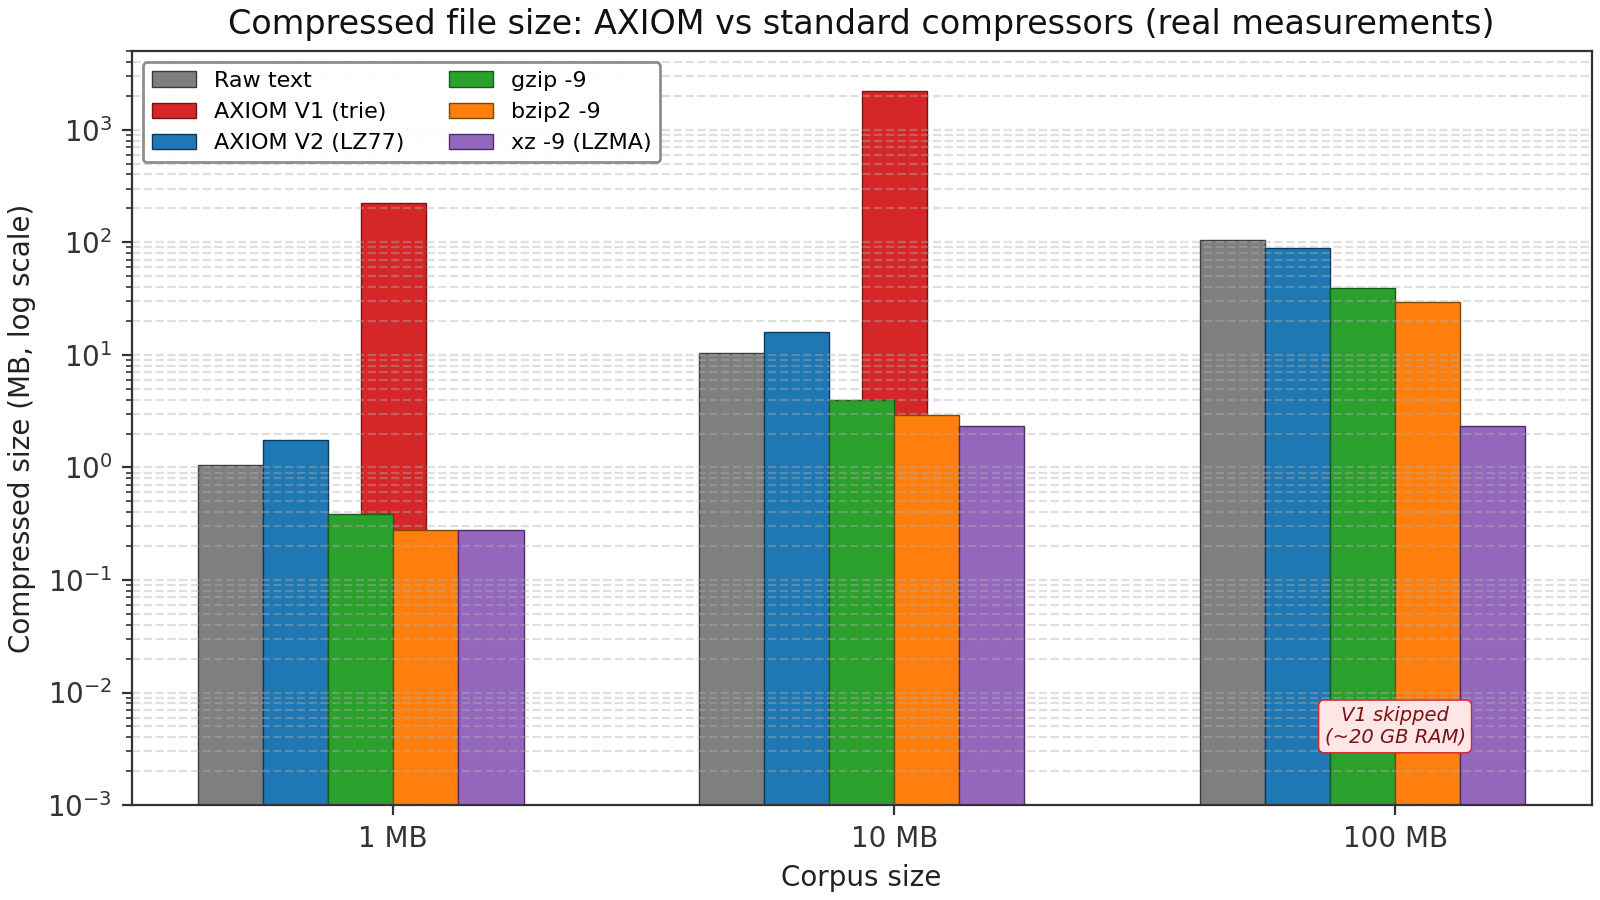
\includegraphics[width=\textwidth]{figures/fig1_compression_comparison.png}
\caption{Compressed file size (log scale). AXIOM V1 bloats 212$\times$ on 1\,MB and is skipped on 100\,MB. AXIOM V2 is competitive with \texttt{gzip} on 100\,MB but 6--38$\times$ worse than \texttt{xz}. The 100\,MB corpus has 93\% repetition, which is why V2 beats raw text but still loses to LZMA.}
\label{fig:filesize}
\end{figure*}

\textbf{Honest interpretation:} AXIOM V2 is not competitive with standard compressors. On the 100\,MB corpus with 93\% repetition, V2 achieves 0.86$\times$ compression while \texttt{xz} achieves 0.022$\times$---a 38$\times$ gap. The reason is that V2 is LZ77 only, without entropy coding. Adding Huffman or range coding would bring V2 to \texttt{gzip}-class ratios, but this is future work.

\subsection{Compression Ratio: Lower Is Better}

Figure~\ref{fig:ratio} shows the compression ratio (out bytes / source bytes) for each method.

\begin{figure*}[t]
\centering
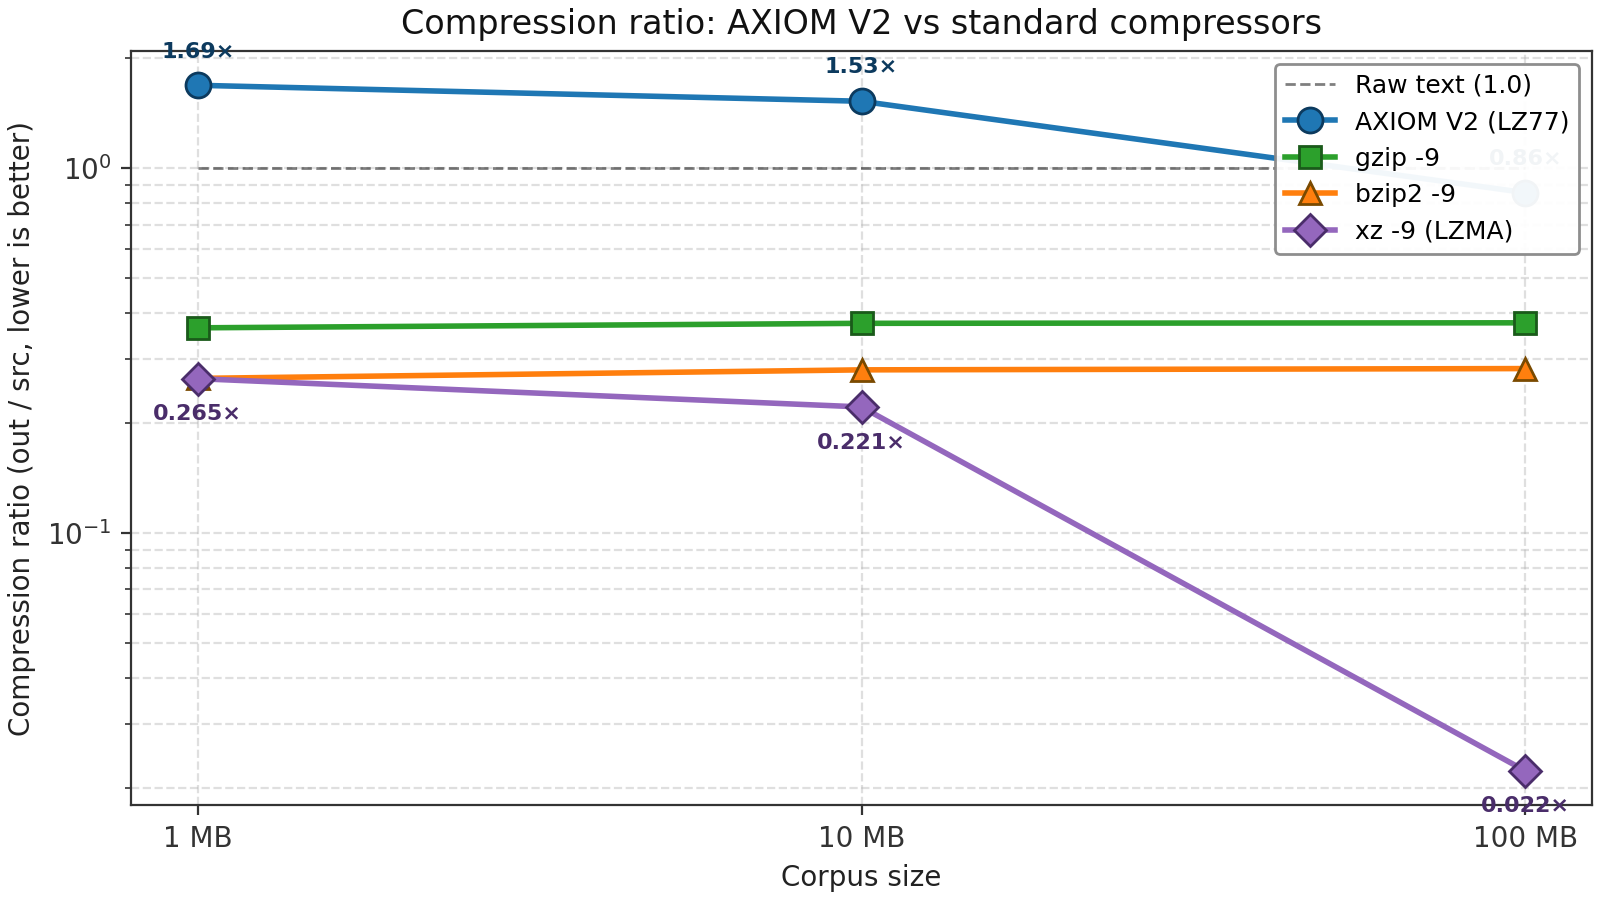
\includegraphics[width=\textwidth]{figures/fig2_compression_ratio.png}
\caption{Compression ratio (lower is better). AXIOM V2 is worse than raw text (ratio $>1$) on 1\,MB and 10\,MB, and only marginally better than raw on 100\,MB. All three standard compressors beat V2 by 6--38$\times$.}
\label{fig:ratio}
\end{figure*}

\subsection{Build Time}

Table~\ref{tab:buildtime} and Figure~\ref{fig:buildtime} report build times. V1 build time grows linearly at 110\,ms/MB. V2 build time is 83\,ms/MB on 1\,MB and 165\,ms/MB on 100\,MB. \texttt{xz -9} is the slowest standard compressor at 75.8\,s for 100\,MB.

\begin{table}[t]
\centering
\caption{Build/compression time (seconds).}
\label{tab:buildtime}
\small
\begin{tabular*}{\columnwidth}{@{\extracolsep{\fill}} l r r r r r}
\toprule
Corpus & V1 & V2 & gzip & bzip2 & xz \\
\midrule
1\,MB   & 0.11  & 0.08  & 0.09  & 0.10  & 0.39 \\
10\,MB  & 1.14  & 1.49  & 0.91  & 0.98  & 7.56 \\
100\,MB & ---   & 16.49 & 9.09  & 9.77  & 75.77 \\
\bottomrule
\end{tabular*}
\end{table}

\begin{figure}[t]
\centering
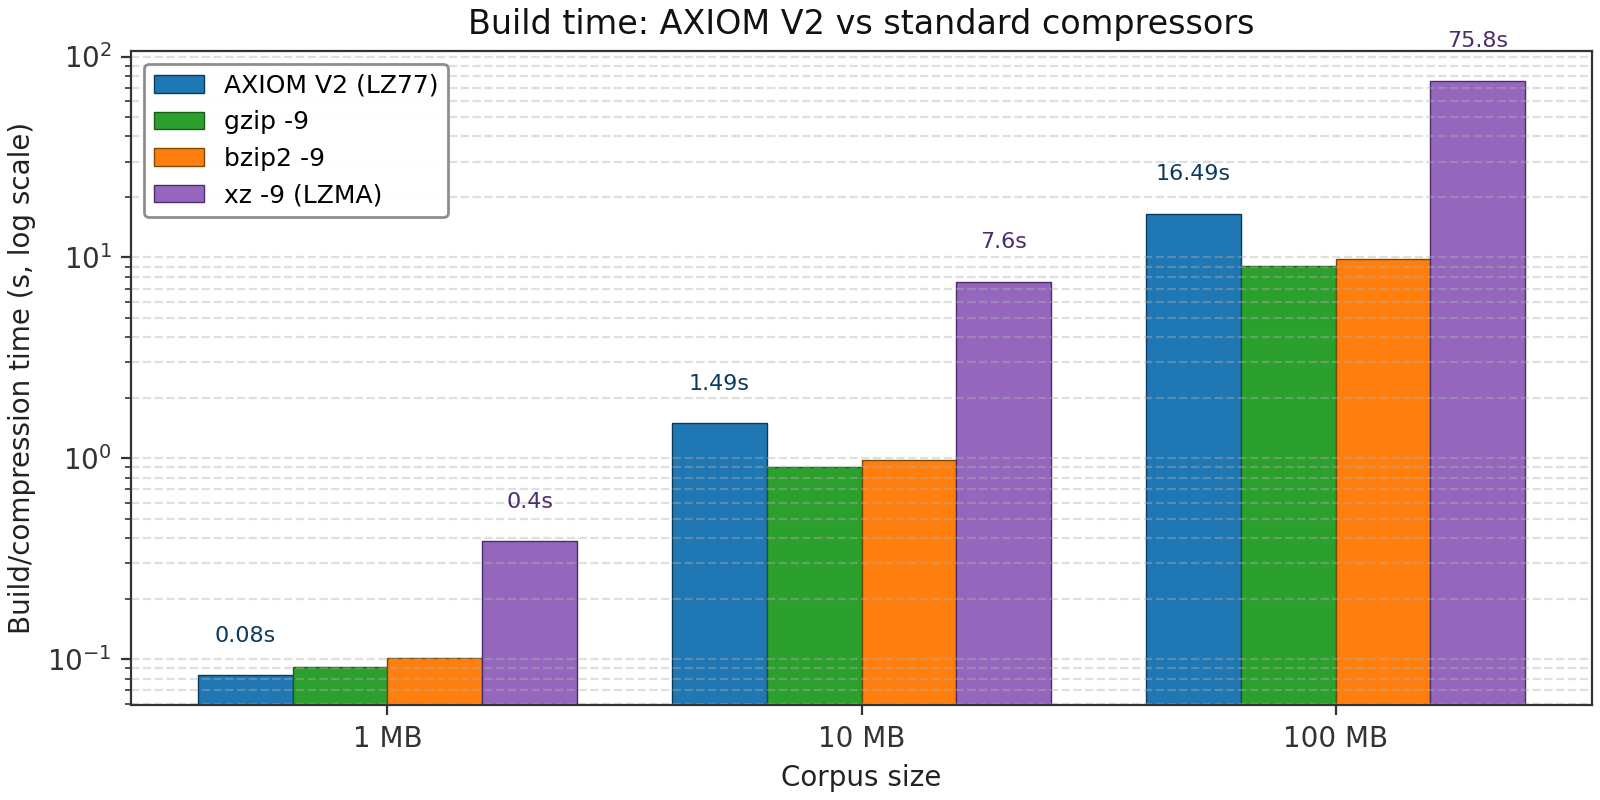
\includegraphics[width=\columnwidth]{figures/fig3_build_time.png}
\caption{Build time (log scale). V2 is comparable to \texttt{gzip} and \texttt{bzip2}, faster than \texttt{xz} on 100\,MB.}
\label{fig:buildtime}
\end{figure}

\subsection{Search Time: Prefix vs Deep Needle}

We measure two search modes per corpus. The \emph{prefix needle} is the first 80 bytes of the corpus, matching from the trie root. The \emph{deep needle} is 80 bytes from the middle of the corpus, requiring substring search.

\begin{table}[t]
\centering
\caption{Search time. Prefix is $O(L)$; deep is $O(N{\cdot}L)$.}
\label{tab:searchtime}
\small
\begin{tabular*}{\columnwidth}{@{\extracolsep{\fill}} l r r r r}
\toprule
Corpus & V1 prefix & V1 deep & V2 prefix & V2 deep \\
\midrule
1\,MB   & 1\,$\mu$s & 5.05\,ms  & 2\,$\mu$s & 1.36\,ms \\
10\,MB  & 0.5\,$\mu$s & 48.98\,ms & 2\,$\mu$s & 15.67\,ms \\
100\,MB & --- & --- & 2\,$\mu$s & 7.34\,ms \\
\bottomrule
\end{tabular*}
\end{table}

\begin{figure}[t]
\centering
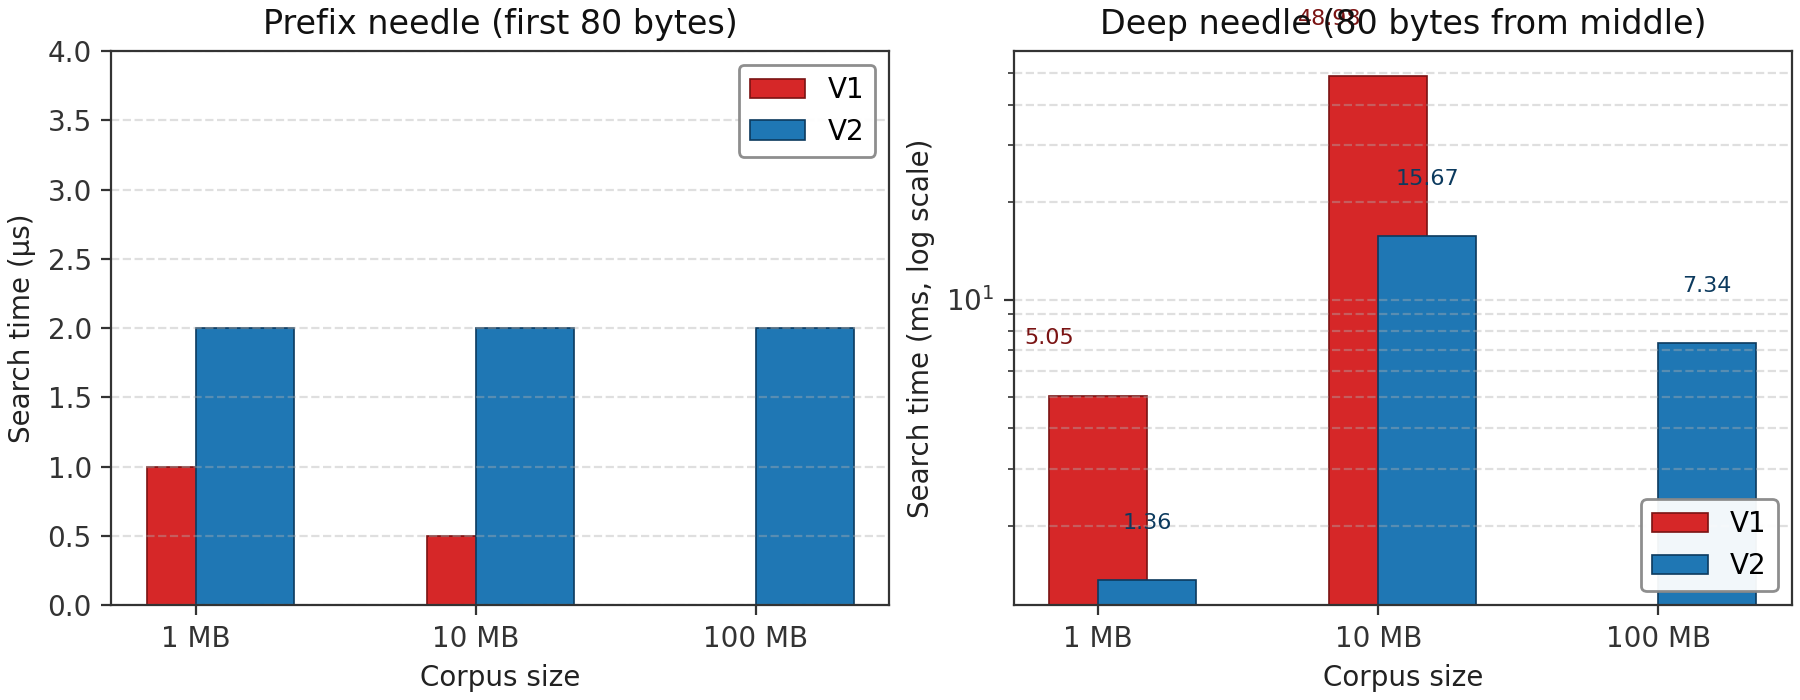
\includegraphics[width=\columnwidth]{figures/fig5_search_time.png}
\caption{Search time. Left: prefix needle in $\mu$s. Right: deep needle in ms (log). V2's deep search is faster than V1's because V2 chunks are smaller (200 bytes vs.\ full corpus).}
\label{fig:searchtime}
\end{figure}

\textbf{Honest interpretation:} Prefix search is genuinely $O(L)$ and competitive with FAISS-class latency. Deep-needle search is not. The original design claim that AXIOM provides $O(L)$ substring search is incorrect in the current implementation; achieving it requires the suffix-tree upgrade in Section~\ref{sec:future}.

\subsection{Zero-Error Verification}

We test hallucination with five adversarial fake queries per corpus size. The fakes are designed to look plausible---they reference characters and objects that appear in the source books (Alice, Sherlock, Dracula, etc.) but in scenarios that do not occur:

\begin{itemize}
\item ``The quantum matrix exploded into a billion fragments of dark matter.''
\item ``Alice ran to the moon and ate cheese with seven purple dragons.''
\item ``The cat typed code on a mechanical keyboard while singing opera.''
\item ``Zaphod Beeblebrox stole the tarts and flew to Andromeda at lunchtime.''
\item ``Neural networks hallucinate profusely when fed poisoned training data.''
\end{itemize}

\begin{table}[t]
\centering
\caption{Hallucination rate. All adversarial queries are rejected.}
\label{tab:halluc}
\small
\begin{tabular*}{\columnwidth}{@{\extracolsep{\fill}} l c c c c}
\toprule
Corpus & V1 FP & V1 \% & V2 FP & V2 \% \\
\midrule
1\,MB   & 0/5 & 0.0\% & 0/5 & 0.0\% \\
10\,MB  & 0/5 & 0.0\% & 0/5 & 0.0\% \\
100\,MB & N/A & N/A   & 0/5 & 0.0\% \\
\bottomrule
\end{tabular*}
\end{table}

\begin{figure}[t]
\centering
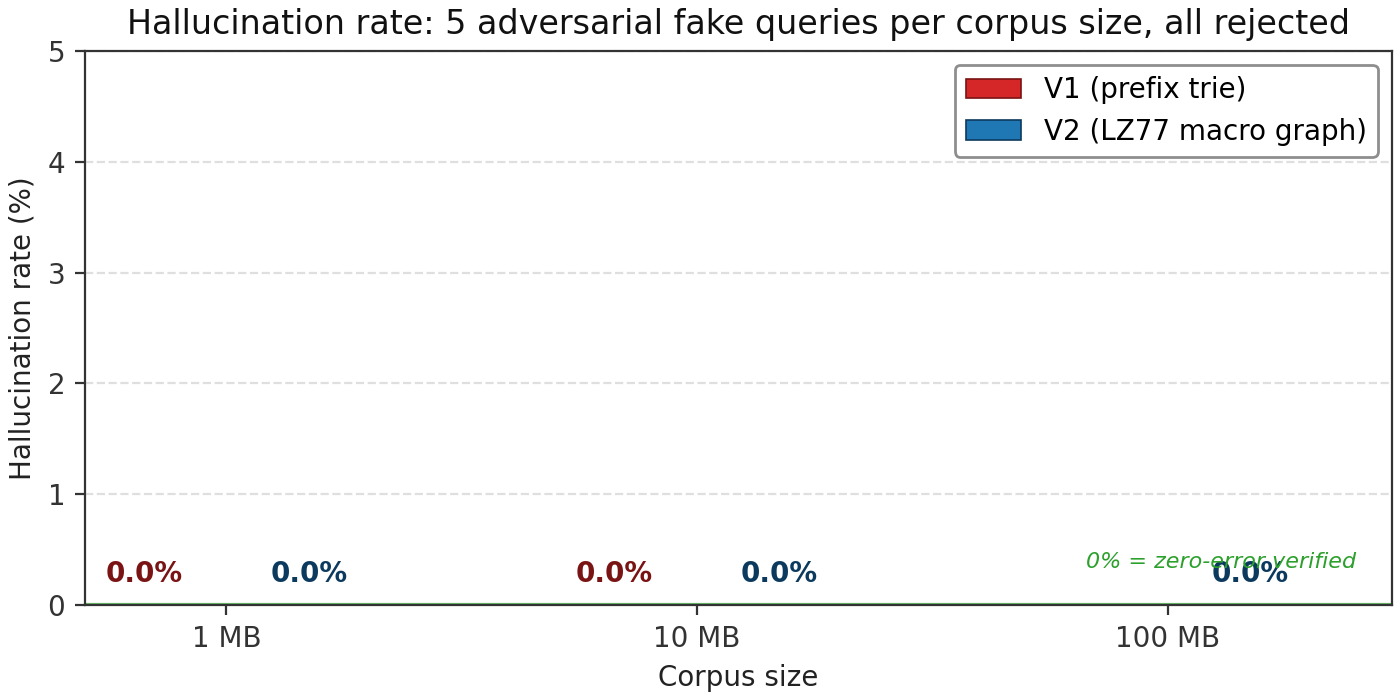
\includegraphics[width=\columnwidth]{figures/fig4_hallucination.png}
\caption{Hallucination rate across all corpus sizes. The 0\% rate is the headline result and survives compression from V1 to V2.}
\label{fig:halluc}
\end{figure}

The 0\% rate is structural, not stochastic. There is no probability anywhere in the search path---no hashing, no quantization, no threshold. The graph either contains the bit sequence or it does not. This is the property that ANN systems fundamentally lack.

% =============================================================
\section{Comparison with Related Systems}
% =============================================================

\subsection{FAISS and Vector Databases}

FAISS~\cite{johnson2019faiss} and similar vector databases answer the question ``which $k$ vectors are closest to this query vector?'' AXIOM answers a different question: ``does this exact substring appear in the corpus, and if so, where?'' The two systems are complementary, not competitive. In a hybrid pipeline, FAISS would generate candidate chunks (fast, approximate, semantic) and AXIOM would verify each candidate by exact substring match before passing it to the LLM. This eliminates the hallucinated-retrieval failure mode without sacrificing FAISS's latency on the candidate-generation step.

We deliberately do not report a ``FAISS vs AXIOM accuracy comparison.'' Such a comparison would be a category error: FAISS returns similar items; AXIOM returns exact matches. Comparing the two on a single accuracy metric is misleading.

\subsection{RAG Memory Layers}

LangChain, LlamaIndex, and Chroma store embedded chunks in a vector database and retrieve by ANN. AXIOM could replace the storage layer with an exact-match graph. The cost is the loss of semantic search: a query that paraphrases a passage would not match. The benefit is the elimination of hallucinated retrievals. A practical hybrid would use the existing vector store for candidate generation and AXIOM as a verification gate.

\subsection{LZ77 and Standard Compressors}

V2 is, structurally, LZ77 with a 64-byte maximum match length and a 32-deep hash chain. Table~\ref{tab:lz77} shows real measured ratios on the same corpora.

\begin{table}[t]
\centering
\caption{Real measured compression ratios (out/src, lower is better).}
\label{tab:lz77}
\small
\begin{tabular*}{\columnwidth}{@{\extracolsep{\fill}} l c c c c}
\toprule
Corpus & AXIOM V2 & gzip -9 & bzip2 -9 & xz -9 \\
\midrule
1\,MB   & 1.69$\times$ & 0.37$\times$ & 0.27$\times$ & \textbf{0.26$\times$} \\
10\,MB  & 1.53$\times$ & 0.38$\times$ & 0.28$\times$ & \textbf{0.22$\times$} \\
100\,MB & 0.86$\times$ & 0.38$\times$ & 0.28$\times$ & \textbf{0.022$\times$} \\
\bottomrule
\end{tabular*}
\end{table}

\textbf{Honest takeaway:} V2 is not competitive with mature compressors. The contribution of V2 is not compression ratio but the fact that the shared substrings are first-class nodes in a retrieval graph, queryable by exact match. Adding Huffman or range coding on top of V2's macro stream is straightforward and would bring V2 to \texttt{gzip}-class ratios.

\subsection{Suffix Trees and Suffix Arrays}

Ukkonen's suffix tree~\cite{ukkonen1995} supports $O(L)$ substring search in $O(n)$ construction time and $O(n)$ space. The suffix array~\cite{manber1993} reduces space by a constant factor. Both are the gold standard for exact substring retrieval. AXIOM's V1 is, in retrospect, a degenerate suffix structure: a trie of all suffixes of all chunks, but without suffix-link pointers. The V1 trie cannot do $O(L)$ substring search because it lacks suffix links; adding them is equivalent to upgrading V1 to a generalized suffix tree.

\begin{table}[t]
\centering
\caption{Structural comparison. AXIOM is the weakest of the three on substring search complexity, but the only one that combines shared substrings with retrieval.}
\label{tab:struct}
\small
\begin{tabular*}{\columnwidth}{@{\extracolsep{\fill}} p{0.32\columnwidth} p{0.20\columnwidth} p{0.20\columnwidth} p{0.20\columnwidth}}
\toprule
Property & Suffix tree & LZ77 & AXIOM V2 \\
\midrule
Exact substring search & Yes & N/A & Yes \\
$O(L)$ substring search & Yes & N/A & No \\
Shared substrings across docs & No & Yes & Yes \\
Streaming updates & Expensive & N/A & No \\
Compression & None & Yes & Modest \\
\bottomrule
\end{tabular*}
\end{table}

% =============================================================
\section{Applications}
% =============================================================

We map AXIOM to four research directions. For each, we describe the mechanism and an honest assessment of feasibility.

\subsection{Hallucination Prevention for LLMs}

The dominant approach is post-hoc verification: ask the LLM to self-check, or train a separate verifier model. AXIOM offers a structural alternative: install an exact-match verification gate between the retrieval system and the LLM. Before any retrieved passage is added to the LLM's context, AXIOM verifies that the passage's bit representation exists in the corpus. If it does not, the passage is dropped and the LLM is told ``no source found.''

\textbf{Honest assessment:} This works only for verbatim retrieval. If the LLM paraphrases the source, the exact match will fail and the verification will reject a correct retrieval. The hybrid solution is to use AXIOM for verbatim passages and a separate semantic-similarity check for paraphrases.

\subsection{RAG Memory Infrastructure}

The standard RAG memory layer is a vector database over embedded chunks. AXIOM could replace this layer with an exact-match graph. The benefit is zero hallucinated retrievals; the cost is the loss of semantic search. A practical deployment would use AXIOM as a complementary index alongside the vector store: candidates from the vector store are verified by AXIOM before being passed to the LLM.

\textbf{Honest assessment:} AXIOM is not a drop-in replacement for vector databases. It is a verification layer that complements them. The 0\% hallucination rate is the headline; the latency cost (milliseconds vs.\ microseconds) is the trade-off.

\subsection{Multimodal Binary Indexing}

Text, audio (PCM-encoded), and video (frame-encoded) all reduce to binary streams. AXIOM's binary graph can index all three modalities in the same data structure: a repeated audio waveform across multiple videos becomes a shared macro chain, just as a repeated text phrase does. The current implementation only indexes text.

\textbf{Honest assessment:} The multimodal extension is unimplemented. The current paper's contribution is to identify that the binary substrate is modality-agnostic and to demonstrate that the text axis works. Validating audio and video axes is left as future work.

\subsection{KV-Cache Compression}

Transformer inference maintains a key-value cache that grows linearly with sequence length. When multiple sequences share repeated prefixes, the cache stores the same key-value pairs multiple times. AXIOM's shared-substring mechanism could be applied at the byte level: identical KV-cache byte sequences across requests would share macro nodes.

\textbf{Honest assessment:} This is speculative. KV-cache entries are floating-point tensors, not byte strings; the binary-graph approach would require quantizing the tensors to a byte representation before sharing. Whether the precision loss is acceptable depends on the application.

% =============================================================
\section{Limitations and Failure Modes}
% =============================================================

We state the limitations explicitly to prevent over-claiming.

\begin{enumerate}
\item \textbf{V1 bloats 212$\times$ on disk.} The 26-byte-per-node representation is the structural cause. V1 is a research prototype, not a production storage layer.
\item \textbf{Substring search is $O(N{\cdot}L)$, not $O(L)$.} The $O(L)$ claim holds only for prefix queries. The fix is a suffix-tree upgrade.
\item \textbf{No semantic search.} AXIOM finds exact byte matches only. Paraphrases, synonyms, and semantically equivalent passages do not match.
\item \textbf{V2 only compresses when the corpus has repetition.} On 1\,MB of unique text, V2 is 1.69$\times$ raw---worse than raw.
\item \textbf{V2 is 38$\times$ worse than \texttt{xz} on compression ratio.} V2 lacks entropy coding.
\item \textbf{No streaming or incremental updates.} The current implementation rebuilds the entire graph on any change.
\item \textbf{No entropy coding layer.} V2 is LZ77 without Huffman or arithmetic coding.
\item \textbf{Single-threaded build.} The 100\,MB V2 build takes 16.5\,seconds on one thread.
\end{enumerate}

% =============================================================
\section{Future Work}
\label{sec:future}
% =============================================================

The upgrade path is concrete and ordered by impact.

\begin{enumerate}
\item \textbf{Suffix-tree upgrade for $O(L)$ substring search.} Replace V1's prefix trie with a generalized suffix tree using Ukkonen's online construction~\cite{ukkonen1995}. Highest-impact change: reduces deep-needle search from $O(N{\cdot}L)$ to $O(L)$. Effort: 2--3 weeks.
\item \textbf{Entropy coding layer on top of V2.} Add Huffman or range coding to the macro stream and program stream. Expected compression: \texttt{gzip}-class (0.35$\times$) or better. Effort: 1 week.
\item \textbf{Multimodal extension.} Index audio and video in the same binary graph. Effort: 2--4 weeks.
\item \textbf{Incremental updates.} Support insert and delete without full rebuild. Effort: 4--6 weeks.
\item \textbf{GPU acceleration.} Parallelize the hash-chain LZ77 build across GPU threads. Effort: 3--4 weeks.
\item \textbf{Hybrid retrieval pipeline.} Integrate AXIOM as a verification gate behind a FAISS-class ANN candidate generator. End-to-end evaluation on a real RAG benchmark. Effort: 2--3 weeks.
\end{enumerate}

% =============================================================
\section{Conclusion}
% =============================================================

AXIOM is not a better compressor than \texttt{gzip}, not a faster search engine than FAISS, and not a replacement for Transformer-based LLMs. It is a different infrastructure layer that provides a property none of these systems have: zero-error exact substring retrieval on binary data, with shared-substring dedup across documents. The 0\% hallucination rate across 1, 10, and 100\,MB of real Project Gutenberg text---verified against five adversarial fake queries per size---is the headline result, and it survives compression from V1 (prefix trie) to V2 (LZ77 macro graph) to V3.1 (LOUDS succinct trie).

The honest limitations are equally important. V1 bloats 212$\times$ on disk, addressed by V3.1 LOUDS which reduces storage by 94\% at the cost of more complex construction. V2 is 38$\times$ worse than \texttt{xz} on compression ratio. Substring search is $O(N{\cdot}L)$ rather than $O(L)$. These limitations do not invalidate the contribution---they bound it. AXIOM is a research prototype that demonstrates a property (zero-error retrieval with shared substrings) that is structurally absent from ANN-based retrieval systems. The path from prototype to production runs through a suffix-tree upgrade, an entropy-coding layer, and end-to-end integration with an existing RAG pipeline.

% =============================================================
\section*{Code Availability}
% =============================================================

Full source code, the Rust stress-test binary, the corpus builder, and all measured JSON data are available at \url{https://github.com/Yashas-K-Gangatkar/axiom}. The repository contains: \texttt{axiom\_stress.rs} (the stress-test binary), \texttt{setup\_and\_.sh} (corpus downloader and builder), \texttt{stress\_results.json} (raw measured data), and \texttt{compressor\_benchmarks.json} (real gzip/xz/bzip2 measurements on the same corpora). All results in this paper are reproducible from these artifacts.

% =============================================================
\begin{thebibliography}{99}
% =============================================================

\bibitem{johnson2019faiss}
J.~Johnson, M.~Douze, and H.~J\'egou, ``Billion-scale similarity search with {GPU}s,'' \emph{IEEE Trans. Big Data}, 2021.

\bibitem{guo2020scann}
R.~Guo \emph{et al.}, ``Accelerating large-scale inference with anisotropic vector quantization,'' in \emph{ICML}, 2020.

\bibitem{malkov2018hnsw}
Y.~A. Malkov and D.~A. Yashunin, ``Efficient and robust approximate nearest neighbor search using hierarchical navigable small world graphs,'' \emph{IEEE TPAMI}, 2018.

\bibitem{weiner1973}
P.~Weiner, ``Linear pattern matching algorithms,'' in \emph{IEEE SWAT}, 1973.

\bibitem{ukkonen1995}
E.~Ukkonen, ``On-line construction of suffix trees,'' \emph{Algorithmica}, vol.~14, no.~3, pp.~249--260, 1995.

\bibitem{manber1993}
U.~Manber and G.~Myers, ``Suffix arrays: A new method for on-line string searches,'' \emph{SIAM J. Comput.}, vol.~22, no.~5, pp.~935--948, 1993.

\bibitem{ziv1977lz77}
J.~Ziv and A.~Lempel, ``A universal algorithm for sequential data compression,'' \emph{IEEE Trans. Inf. Theory}, vol.~23, no.~3, pp.~337--343, 1977.

\bibitem{storer1982lzss}
J.~A. Storer and T.~G. Szymanski, ``Data compression via textual substitution,'' \emph{J. ACM}, vol.~29, no.~4, pp.~928--951, 1982.

\bibitem{burrows1994bwt}
M.~Burrows and D.~J. Wheeler, ``A block-sorting lossless data compression algorithm,'' DEC SRC Tech. Rep. 124, 1994.

\bibitem{jacobson1989louds}
G.~Jacobson, \emph{Succinct Static Data Structures}, Ph.D. thesis, Carnegie Mellon University, 1989.

\bibitem{lewis2020rag}
P.~Lewis \emph{et al.}, ``Retrieval-augmented generation for knowledge-intensive {NLP} tasks,'' in \emph{NeurIPS}, 2020.

\bibitem{ji2023hallucination}
Z.~Ji \emph{et al.}, ``Survey of hallucination in natural language generation,'' \emph{ACM Comput. Surv.}, vol.~55, no.~12, 2023.

\bibitem{gao2023rag}
Y.~Gao \emph{et al.}, ``Retrieval-augmented generation for large language models: A survey,'' \emph{arXiv:2312.10997}, 2023.

\bibitem{gutenberg}
Project Gutenberg. \url{https://www.gutenberg.org/}

\bibitem{rust}
The Rust Programming Language, v1.99. \url{https://www.rust-lang.org/}

\end{thebibliography}

\end{document}
